\documentclass[12pt]{article}
\usepackage[utf8]{inputenc}
% Deutsch: https://de.overleaf.com/learn/German
% "`	Left double quotes
% "'	Right double quotes
\usepackage[T1]{fontenc}
\usepackage[ngerman]{babel}
\usepackage{csquotes}

\usepackage{xcolor}
\usepackage{listings}

\usepackage{tikz}
\usetikzlibrary{positioning,automata}

\usepackage[acronym,nonumberlist]{glossaries}
\usepackage{acronym}

% documentation: https://ctan.kako-dev.de/macros/latex/contrib/biblatex/doc/biblatex.pdf
\usepackage[backend=biber,style=numeric,sorting=ynt]{biblatex}
\addbibresource{references.bib}

% um Grafiken einzubinden, {Angabe des Pfades der Bilder}
\usepackage{float}
\usepackage{graphicx}
\graphicspath{ {images/} }
% Nützliches Online Tool zur Tabellengenerierung: TablesGenerator.com 

% zur korreten Platzierung der Bilder im Titelblatt
\usepackage{chngpage}
\usepackage{calc}
\usepackage{geometry}

% Automatisches Generieren von Hyperlinks bei Verweisen (ref / cite)
\usepackage{hyperref}
\hypersetup{
  colorlinks   = true,    % Colours links instead of ugly boxes
  urlcolor     = blue,    % Colour for external hyperlinks
  linkcolor    = black,    % Colour of internal links
  citecolor    = red      % Colour of citations
}

% Infos über Dokument
\title{Semantic Web}
\author{Sebastian Pötter}
\date{\today}

\begin{document}

    \newgeometry{top=2cm,bottom=2cm}

\begin{titlepage}
    
    \begin{figure}[t]
        \begin{adjustwidth}{-\oddsidemargin-1in}{-\rightmargin}
            \centering
            
\includegraphics[width=\paperwidth]{banner_top}
        \end{adjustwidth}
    \end{figure}

    \begin{flushleft}
        \vspace*{1cm}
        \Huge
        \textbf{Semantic Web}
        
        \vspace{0.5cm}
        \LARGE
        Investitionen in grüne Energie der Bundesregierung Deutschland
        
        \vspace{1.5cm}
        \textbf{Sebastian Pötter}
        
        \vspace{0.5cm}
        \large
        Jahrgang: 20INM
        
        \vspace{0.5cm}
        im Studiengang\\
        Informatik Master
        
    \end{flushleft}        

    \vspace{0.5cm}
    \begin{flushright}
        Semantic Web\\
        Prof. Thomas Riechert\\
        \vspace{0.5cm}
        \today
    \end{flushright}    
    
    \begin{figure}[b]
        \begin{adjustwidth}{-\oddsidemargin-1in}{-\rightmargin}
            \centering
        \end{adjustwidth}
    \end{figure}

\end{titlepage}

\restoregeometry
    \newpage
    
    \pagenumbering{roman}

    \tableofcontents
    
    \newpage
        
    %\addcontentsline{toc}{section}{Abkürzungsverzeichnis}  
    %\section*{Abkürzungsverzeichnis}
    %    \begin{acronym}
    %        \acro {PWA} {Progressive Web Apps}
    %    \end{acronym}
    
    %\newpage
    
    \pagenumbering{arabic}
    
    \section{Einleitung}
    
Im Rahmen des Moduls 'Semantik Web' soll sich mit einer Forschungsfrage beschäftigt werden, diese soll anhand von Datenquellen untersucht werden. Dabei sollen mindestens drei unabhängige Datenquellen benutzt werden, welche logisch miteinander verbunden werden sollen. Falls die Daten dabei noch nicht im RDF Form sind, müssen diese erst um konvertiert und in eine Orthologie eingearbeitet werden. Die Forschungsfrage ist folgende: \textbf{Besteht eine Korrelation zwischen der zurzeit regierenden Parteien in Deutschland und deren Investitionshöhe in erneuerbaren Energien und wie hat sich der Anteil an erneuerbaren Energien im Zeitraum von 2000 bis 2020 verändert? }. Hierfür werden Daten der Wahl und die der regierenden Parteien sowie die Investition und Anteile der erneuerbaren Energien in Deutschland benötigt. 

    \section{Datenquellen}

Um die Forschungsfrage bearbeiten zu können, müssen Daten gefunden werden, welche zu dem Thema passen und aussagekräftig sind. Betrachtet werden Daten im Zeitraum von 2004 bis 2020. Für diesen Zeitraum ist ab 2004 der Aufbau der europäischen Struktur- und Investitionsfonds dokumentiert, hierbei sind auch Daten über Deutschland vorhanden. Da die Bundestagswahl nur aller vier Jahre stattfindet, werden die Zwischenergebnisse durch die Sonntags-frage der Bundestagswahl repräsentiert.

        \subsection{Verteilung der Erzeugung}
'Energy charts' ist eine Seite welche sich mit Themen rund um erneuerbaren Energie beschäftigt (02.07.2021).\\
\\
\vspace{0.5cm}
\begin{tabular}{l|p{9cm}}
	Link & \url{https://www.energy-charts.info/charts/energy/chart.htm?l=de&c=DE&stacking=grouped} \\
 	Datenformat & CSV \\
 	Schnittstelle & HTTPS\\
 	Lizenz & Creative  Commons Attribution 4.0 International \\
 	Open Data & $\star\star\star $ \\
\end{tabular}
\\

\subsection{Wahlen in Deutschland bis 2017}
    Bundestag.de ist eine offizielle Webseite der Bundesregierung Deutschland, welche sich mit dem Thema rund um die Wahl beschäftigt (02.07.2021).\\
\\
\vspace{0.5cm}
\begin{tabular}{l|p{9cm}}
	Link & \url{https://www.bundestag.de/parlament/wahlen/ergebnisse_seit1949-244692} \\
 	Datenformat & HTML \\
 	Schnittstelle & HTTPS\\
 	Lizenz & Creative  Commons Attribution 4.0 International \\
 	Open Data & $\star\star $ \\
\end{tabular}
\\
\subsection{Investition in erneuerbaren Energie bis 2020}
    Offielle Unter-Seite des Ministerium für Wirtschaft und Energie, welches zur Bundesregierung Deutschland gehört.  (02.07.2021).\\
\\
\vspace{0.5cm}
\begin{tabular}{l|p{9cm}}
	Link & \url{https://www.erneuerbare-energien.de/EE/Navigation/DE/Service/Erneuerbare_Energien_in_Zahlen/Entwicklung/entwicklung-der-erneuerbaren-energien-in-deutschland.html} \\
 	Datenformat & Bild \\
 	Schnittstelle & HTTPS\\
 	Lizenz & Creative  Commons Attribution 4.0 International \\
 	Open Data & $\star $ \\
\end{tabular}

\newpage
  
\subsection{Investitionen in Erzeugungsanlagen}
    Stratista ist für eine Webseite, welche alle möglichen Stratistiken sammeln und teilweise kostenlos anbieten.\\
\\
\vspace{0.5cm}
\begin{tabular}{l|p{9cm}}
	Link & \url{https://de.statista.com/statistik/daten/studie/171896/umfrage/investitionen-in-anlagen-zur-nutzung-von-strom-aus-erneuerbaren-energien} \\
 	Datenformat & CSV \\
 	Schnittstelle & HTTPS\\
 	Lizenz & Creative  Commons Attribution 4.0 International \\
 	Open Data & $\star \star \star $ \\
\end{tabular}
  \\  
    \section{Arbeitsvorgang}

Um folgenden soll der Vorgang von den zugrundeliegenden Daten, dessen Suche und Aufbereitung und letztendliche Einarbeitung in das RDF-Schema vorgestellt werden. Hierbei wird auch auf die Erstellung einer eigenen Orthologie auf Grundlagen der Daten eingegangen sowie welche Tools dazu eingesetzt wurden. 

        \subsection{Datensuche}
        
Zu aller erst müssen passende Daten gefunden werden, welche zur Forschungsfrage passen und welche zur Beantwortung dieser Frage beitragen könnten. Hierbei wurde zuerst nach de Wahlergebnissen der Bundesregierung in Deutschland gesucht. Die Bundesregierung besitzt extra ein Archiv, welche genau diese Daten beinhalten, jedoch nur in Tabellenform. Da die Bundesregierung nur aller vier Jahre gewählt wird und zwischenzeitliche keine Daten über die Wahlergebnisse vorhanden sind, müssen die zeitlichen Räume während dieser vier Jahre mit Umfrage-Werten aufgefüllt werden. Hierfür wurden die Daten der Sonntagsfrage der ARD welche monatlich Umfragen über die Wahl der Bundesregierung durchführt. Diese Daten gilt es jetzt nur zu verknüpfen um so Daten in einem vollständigen Zeitraum zu besitzen. Nachdem diese Daten eine Auskunft über die Wahlergebnisse gibt, müssen nun noch Daten über die Investition der Bundesregierung in erneuerbaren Energien und der Gesamtanteil der erneuerbaren Energien gefunden werden. Die Daten, wie viel Investiert wird, konnte auf einer Webseite der Bundesregierung selbst gefunden werden. Leider lagen die Daten nur grafisch vor, sodass diese noch aus dem Bild abgeschrieben werde mussten. Wie hoch nun der Anteil der Erneuerbaren Energien am gesamt Erzeugnisse ist, konnte jedoch nicht in diesen Daten gefunden werden, weshalb hierfür weiter gesucht werden musste. Diese Daten besitzt die Europäische Seite, welche eine vielzahl an Daten anbietet. Somit sind genug Daten vorhanden, um die Forschungsfrage bearbeiten zu können.
        
        \subsection{Datenbereinigung}
        
Um die gefundenen Daten nun einpflegen zu können müssen diese erst bereinigt werden. Da fast alle Daten als Tabelle vorlagen (CSV) musste hierfür nur wenig getan werden, außer die Daten der Investition aus der Grafik in eine Tabelle zu übertragen. Zusätzlich mussten Sonderzeichen oder Umlaute wie ÄÖÜ ersetzt werden, da es sonst zu Problemen im RDF-Schema kommen kann. Da die Daten von der Europäischen Union noch unter anderem Daten über Kohle-kraft und Atom-kraft beinhielten mussten diese Spalten aus der Tabelle gelöscht werden, da diese irrelevant für die Forschungsfrage waren. Genauso müssen Leerzeichen, Slashes und Back-Slashes entfernt, oder durch passende Zeichen ersetzt werden. Nachdem die Daten bereinigt wurden, müssen diese noch so umbenannt werden, dass Zusammenhängende Daten auch als solche erkannt werden können. Beispielsweise 'Wasserkaft' hieß in der einen Datenquelle 'Wasserkraft' und in anderen 'Wasserkraft und Wassererzeugnisse', solche müssten auf die selben Wörter unbenannt werden, sodass es möglich ist auch verknüpfte Anfragen zu stellen, welche z.B. Investition und Erzeugungsanteil ausgibt. Auch bei den Daten der Wahlergebnisse und der Wahlprognosen gab es Unterschiede, da sich einzelnen Parteien in Laufe der Zeit unbenannt hatten. Ein weiteres Problem war die Angabe der Zahlen, welche bei der Kommastelle ein Komma besitzt und diese aber im RDF-Format mit einem Punkt gekennzeichnet werden muss, da die Zahl sonst fehlinterpretiert wird, beziehungsweise es zu Fehlern im Importvorgang kommt. 

        \subsection{Orthologie}
    
\begin{figure}[!ht]
    \caption{Entwickelte Orthologie}
    \centering
    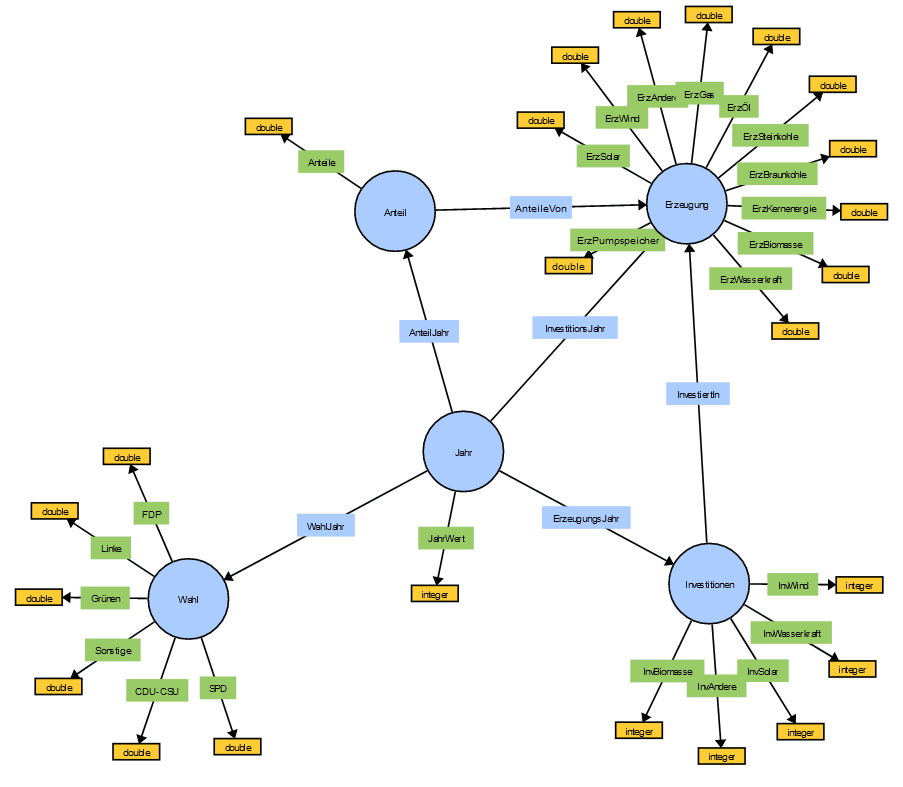
\includegraphics[width=1.2\textwidth]{images/orthologie.png}
    \label{fig:orthologie}
\end{figure}

Da keine der Daten in einer RDF Form sind, muss zunächst eine eigene Orthologie entwickelt und diese Daten dann mit der Orthologie verbunden werden. Zum erstellen der Orthologie wird hierfür wurde das Tool Visual Data Web verwendet. Welche als Webseite zur Verfügung steht und kostenlos nutzbar ist. In Tabelle \ref{fig:table} kann das Vokabular der Orthologie betrachtet werden. 
    
\begin{table}[]
\caption{SPO - Aufbau der Orthologie}
\begin{tabular}{|l|l|l|}
\hline
\textbf{Subjekt} & \textbf{Prädikat} & \textbf{Objekt} \\ \hline
Jahr             & AnteilJahr        & Anteil          \\ \hline
Jahr             & InvestionJahr     & Investitionen   \\ \hline
Jahr             & ErzeugungsJahr    & Erzeugung       \\ \hline
Jahr             & Wahljahr          & Wahl            \\ \hline
Investitionen    & InvestiertIn      & Erzeugung       \\ \hline
Anteil           & AnteilVon         & Erzeugung       \\ \hline
\end{tabular}
\label{fig:table}
\end{table}

        \subsubsection{Visual Data Web}
        
Visual Data Web biete die Möglichkeit eine Orthologie zu visualisieren, oder eine graphisch zu entwickeln. Um eine Orthologie zu erstellen muss der Bearbeitungs-Modus aktiv sein. Im Bearbeitungs-Modus können neue Klassen hinzugefügt werden. Dabei ist es auch möglich einer Klasse eine Eigenschaft zuzuweisen und welche Datentyp diese Eigenschaft hat. Wurde die Orthologie fertiggestellt, so ist es möglich diese als Bild oder als JSON-Datei zu exportieren. 
        
        \subsubsection{Datenabhängigkeit}
    
Alle Daten sollen über das Jahr gefunden und verknüpft werden. Hierfür ist es notwendig, dass die Daten eine Zeiteinheit benötigen, sodass diese mit dem Jahr verknüpft werden können. Da sich die Datenquellen sowie so auf die Zeitliche Veränderungen von Daten beziehen ist es nicht mehr nötig, diese manuell mit einem Zeitpunkt zu versehen. Auf Grundlage der Daten konnte die Die Orthologie erstellt werden, welche mit der Abbildung \ref{fig:orthologie} übereinstimmt. Diese besitzt das Jahr als Schnittstelle für alle anderen Daten, welche mit in der Orthologie enthalten sind. Um die Daten der Wahlergebnisse darstelle zu können wurde eine Klasse 'Wahl' erstellt, welche Jahr und die Anteile der Parteien enthielten und den Typ Zahl hatten. Die Anteile der Erneuerbaren Energien anhand der Gesamt-Erzeugung wurden in einer eignen Klasse gespeichert und nicht selbst berechnet, da sich der Anteil so einfacher abfragen lässt. Die Beträge der Investitionen in erneuerbaren Energien wurden als Double-Wert in der Klasse 'Investition' gespeichert und zusammen mit der Klasse 'Erzeugung' sowie 'Jahr' verknüpft. Die Daten der Erzeugung wurden in der selben namigen Klasse gespeichert und mit 'Anteil', 'Jahr' und 'Investition' verknüpft. Somit konnte eine Orthologie erstellen werden, welche genau zu den Daten passen und eine Abfrage so einfach wie möglich machen sollte.
    

        \subsection{Konvertierung der Daten ins RDF Format}
        
Da nun alle Daten bereinigt vorliegen und eine Orthologie als Struktur exisitiert, kann damit begonnen werden die Daten vom CSV Format in das RDF Format zu konvertieren. Dies konnte mithilfe der Programme 'GraphDB' und 'Protégé' umgesetzt werden. Die Anwendung 'Protégé' ist ein kosnteloses quelloffenes Programm, welche für das Erstellen der Semantik benutzt wird. 'GraphDB' ist eine kostenpflichtige Anwendung, welche aber eine Test-Version besitzt und ist für Studenten bis zu 30 Tage kostenlos nutzbar. Dieses Tool soll für die SPARQL-Abfage benutzt werden und benötigt hierfür die Daten in CSV-Format und die Semantik von 'Protégé'.

            \subsubsection{Protégé}

'Protégé' ist eine freie, quelloffene Plattform, die einer wachsenden Nutzergemeinschaft eine Reihe von Werkzeugen zur Verfügung stellt, um Domänenmodelle und wissensbasierte Anwendungen mit Ontologien zu erstellen. Hierfür kann die erstellte Orthologie von 'Visual Data Web' importiert werden. Trotzdem müssen die Klassen nochmals angepasst und die Eigenschaften hinzugefügt werden. Zu Letzt kann die erstellte Struktur expotiert werden, sodass diese in 'GraphDB' benutzt werden kann um die Daten importieren und mit einer SPARQL-Abfrage ausgeben zu können. Im folgenden werden die Arbeitsschritte an einem Beispiel vorgestellt.

Zu aller erst muss für jede Tabelle eine Klasse erstellt werden. Aus den Datenquellen ergeben sich somit fünf Klassen. Diese haben alle die Elternklasse 'Thing', welche die standard Klasse ist und bereits über ein paar Eigenschaften verfügt. 

\begin{figure}[!ht]
    \caption{Protégé - Klassenansicht}
    \centering
    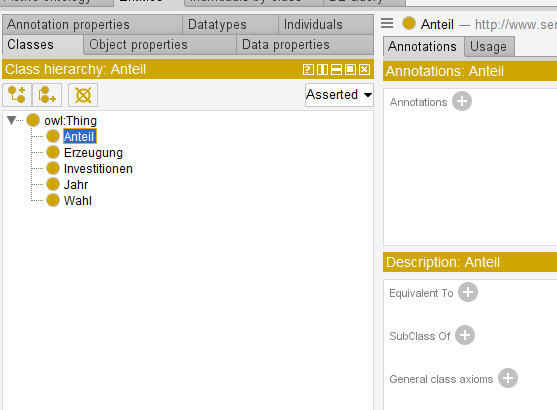
\includegraphics[width=0.8\textwidth]{images/protege_1.png}
    \label{fig:class}
\end{figure}

Die angelegten Klassen müssen noch über Eigenschaften miteinander verbunden werden. Diese Eigenschaft soft dafür, dass in den Anfragen später ein korrektes verlinken der Quellen funktioniert. 

\begin{figure}[!ht]
    \caption{Protégé - Verbindung der Klassen}
    \centering
    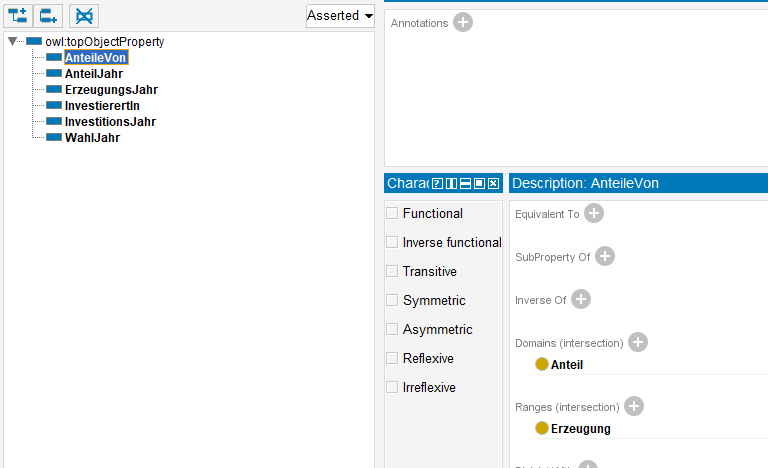
\includegraphics[width=0.8\textwidth]{images/protege_2.png}
    \label{fig:classRelation}
\end{figure}

Zuletzt muss die Orthologie noch exportiert werden. Auch hier gibt es die Möglichkeit verschiedene Datenformate auszuwählen (JSON, TXT, OWL und viele mehr), da aber Graphdb verwendet wird, muss es zwingend das OWL-Format sein. Die W3C Web Ontology Language (OWL) ist eine Sprache des Semantic Web, mit der sich umfangreiches und komplexes Wissen über Dinge, Gruppen von Dingen und Beziehungen zwischen Dingen darstellen lässt. OWL ist eine auf Computerlogik basierende Sprache, so dass das in OWL ausgedrückte Wissen von Computerprogrammen genutzt werden kann, z. B. um die Konsistenz dieses Wissens zu überprüfen oder um implizites Wissen explizit zu machen.

            \subsubsection{GraphDB}
            
Dieses Kapitel beschreibt die Arbeitsvorgänge mit GraphDB von dem Import der OWL-Datei sowie der Import der Daten aus den CSV-Dateien. 'GraphDB' ist eine Graphen-Datenbank und ein Knowledge-Discovery-Tool, das RDF- und SPARQL-kompatibel ist und als Hochverfügbarkeits-Cluster zur Verfügung steht. 'Ontotext GraphDB' wird in verschiedenen europäischen Forschungsprojekten eingesetzt. Im April 2021 ist Graph DB der viert beliebteste RDF-Speicher und das sechst beliebteste DBMS-System in Europa. 

Zunächst muss die OWL-Struktur importiert werde. Dach können die CSV-Daten Importiert werden (siehe Abbildung \ref{fig:graphimport}).

\begin{figure}[!ht]
    \caption{GraphDB - Import der TTL-Daten}
    \centering
    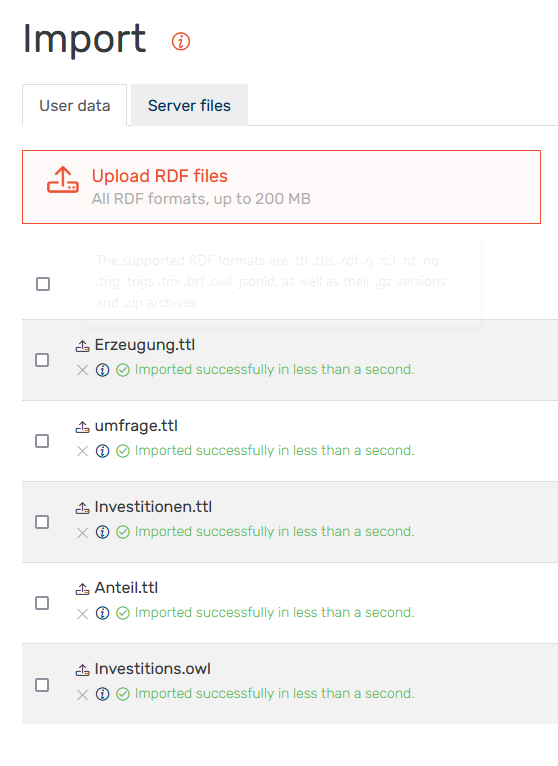
\includegraphics[width=0.6\textwidth]{images/graphdb_1.png}
    \label{fig:graphimport}
\end{figure}

Es wird 'OntoRefine' von 'GraphDB' benutzt um die Daten aus den CSV-Dateien in die Ortholigie zu laden und mit der Sturktur zu verbinden (siehe Abbilding \ref{fig:graphrefine}).

\newpage

\begin{figure}[!ht]
    \caption{GraphDB - Verbindung der Klassen}
    \centering
    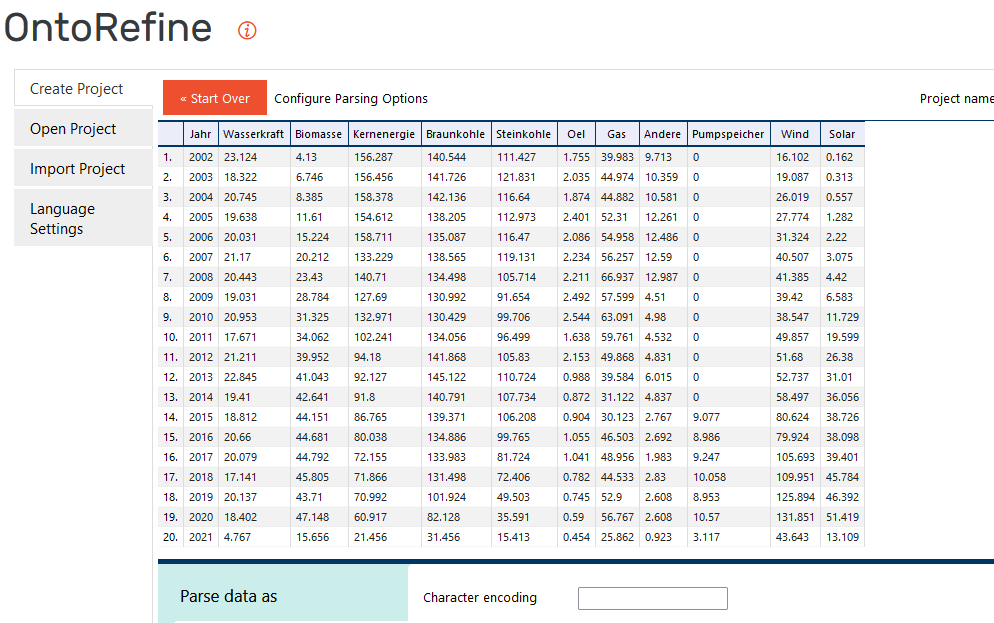
\includegraphics[width=0.8\textwidth]{images/graphdb_2.png}
    \label{fig:graphrefine}
\end{figure}

 Diese müssen nun noch mit der OWL-Struktur verknüpft werden. Die Verlinkung der einzelnen Daten, erfolgt durch den Verweis auf die Spalten, der importieren CSV-Dateien, unter der Verwendung von IRI's. Die Verlinkung der unterschiedlichen Datenquellen erfolgt über die namens gleiche und Inhalt überschneidende Spalte: 'Jahr', welche auf Abbildung \ref{fig:graphrefine-2} zu sehen ist. Dies erfolgt automatisch für Datenquellen mit derselben Basis-IRI mithilfe von GraphDB.

\begin{figure}[!ht]
    \caption{GraphDB - Verknüpfung der Elemente}
    \centering
    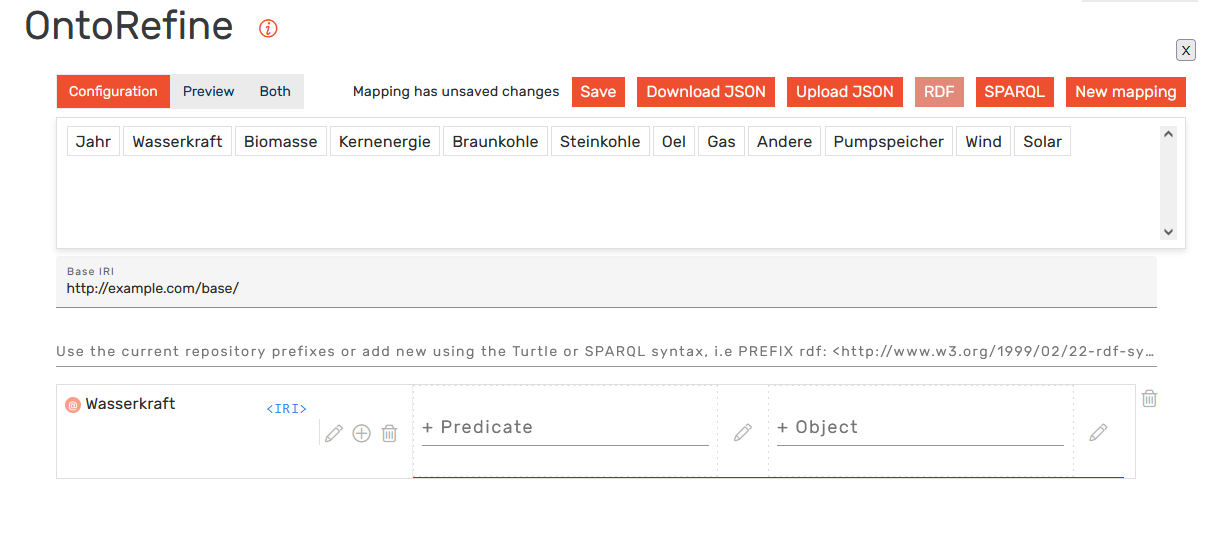
\includegraphics[width=0.8\textwidth]{images/graphdb_3.png}
    \label{fig:graphrefine-2}
\end{figure}

\newpage

    \section{SPARQL Anfragen}
    
Folgende Anfragen dienen der Veranschaulichung der Daten, welche nun im RDF-Format vorliegen und ein eigenes Vokabular besitzen. Es sollen zu erst alle Investitionen im Zeitraum von 2004-2020 ausgegeben werden und danach die der Wahl im selben Zeitraum. Zusätzlich sollen die Investition in erneuerbare Energien gegenüber der Erzeugung von erneuerbare Energien, sowie dessen Anteil an der Gesamterzeugung gestellt werden.

\begin{lstlisting}[language=sql]
@prefix owo: <http://www.semanticweb.org/Sebastian/> .

SELECT ?JahrWert ?ErzAndere ?ErzGas ?ErzBraunkohle ?ErzKernenergie
?ErzPumpspeicher ?ErzSolar ?ErzSteinkohle ?ErzWasserkraft
?ErzWind ?ErzOel ?ErzBiomasse ?SPD ?Sonstige as ?SonstigeWaehler
?Linke ?FDP ?Gruenen ?InvAndere ?InvBiomasse ?InvSolar ?InvWasserkraft
?InvWind ?JahrWert

WHERE
{
	?Jahr owo:AnteilJahr ? Anteil .
	?Jahr owo:InvestitionsJahr ? Investitionen .
	?Jahr owo:ErzeugungJahr ? Erzeugung .
	?Jahr owo:WahlJahr ? Wahl .
	
	?Anteil rdf:type owo:Anteil .
	?Anteil owo:AnteileVon ?Erzeugung .
	?Investitionen rdf:type owo:Investitionen .
	?Investitionen owo:InvestitiertIn  ?Erzeugung.
	?Erzeugung rdf:type owo:Erzeugung .
	?Wahl rdf:type owo:Wahl .
	?Jahr rdf:type owo:Jahr .
	
	FILTER(xsd:integer (?JahrWert) => 2004) . 
	FILTER(xsd:integer (?JahrWert) < 2021) .
}

GROUP By ?JahrWert

ORDER By ASC ?JahrWert
\end{lstlisting}

Als letztes sollen die Daten der Investitionen und die der Wahlen gegenübergestellt werden. Hierbei wird der Zeitraum von 2000 bis 2010 betrachtet. Hierfür müssen nur die anderen Abfrage-Werte entfernt und der Zeitraum angepasst werden.

\begin{lstlisting}[language=sql]
@prefix owo: <http://www.semanticweb.org/Sebastian/> .

SELECT ?JahrWert ?SPD ?Linke ?FDP ?Gruenen 
?Sonstige as ?SonstigeWaehler ?InvAndere ?InvBiomasse 
?InvSolar ?InvWasserkraft ?InvWind ?JahrWert

WHERE
{
	?Jahr owo:InvestitionsJahr ? Investitionen .
	?Jahr owo:WahlJahr ? Wahl .

	?Investitionen rdf:type owo:Investitionen .
	?Investitionen owo:InvestitiertIn  ?Erzeugung .
	?Wahl rdf:type owo:Wahl .
	?Jahr rdf:type owo:Jahr .
	
	FILTER(xsd:integer (?JahrWert) => 2000) . 
	FILTER(xsd:integer (?JahrWert) < 2010) .
}

GROUP By ?JahrWert

ORDER By ASC ?JahrWert
\end{lstlisting}

        \subsection{Diagramme zeichnen}

Als letztes werden die aus den Anfragen erzeugten Daten noch in Diagramme umgewandelt werden. Dies wurde mit Microsoft Excel bewerkstelligt werden. Hierfür werden die Daten der SPARQL-Anfrage als CSV exportiert und in Excel geladen. Im folgenden werden diese Diagramme kurz vorgestellt. Abbildung \ref{fig:dia-wahl} zeigt den Wahlverlauf von 2004 bis 2020 und zusätzlich die Gewählte Bundesregierung zu dieser Zeit. Dabei entspricht Grün: Die GRÜNEN, Geld: FDP, Rot: SPD und Schwarz:CDU. Diese Daten wurden nachträglich hinzugefügt, zum besserem Verständnisse.

\begin{figure}[!ht]
    \caption{Wahlverlauf}
    \centering
    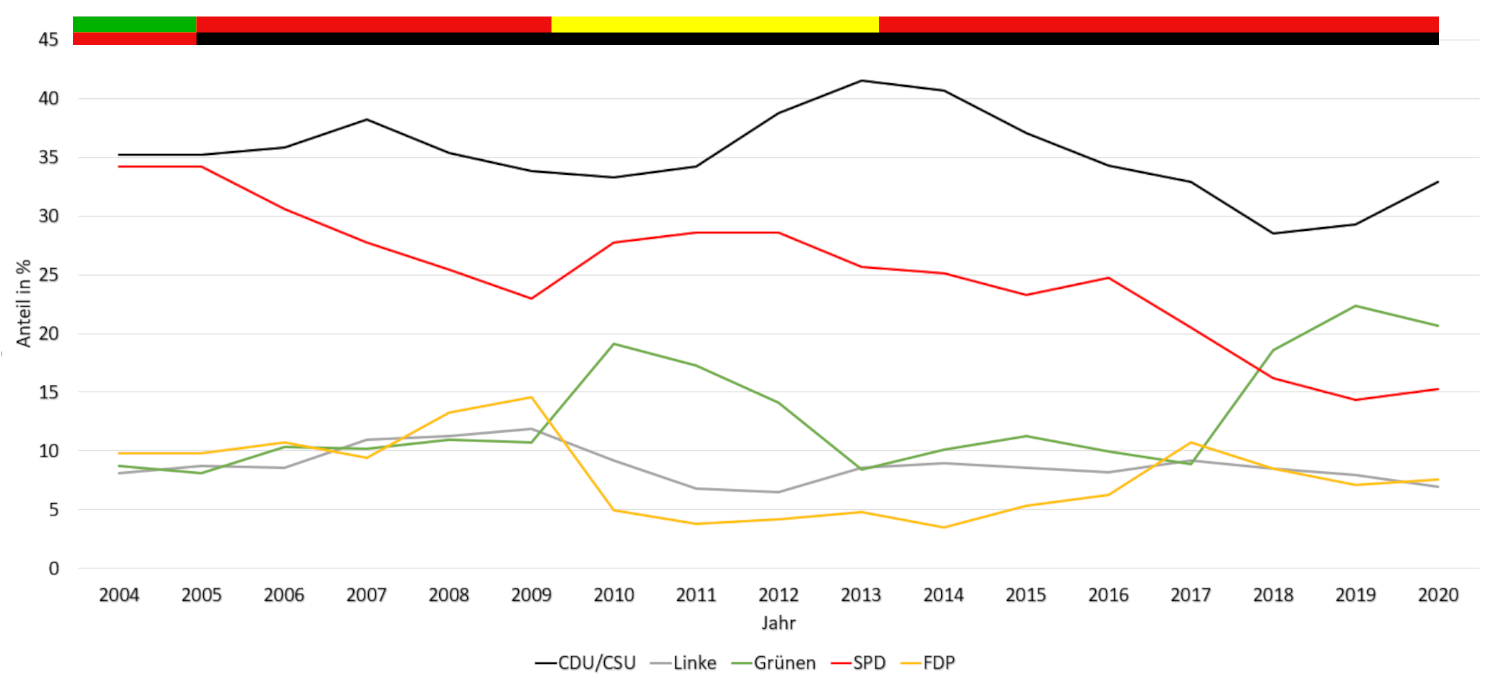
\includegraphics[width=1\textwidth]{images/dia_1.png}
    \label{fig:dia-wahl}
\end{figure}

Das Diagramm von Abbildung \ref{fig:dia-invest} visualisiert die Investitionen der Bundesregierung Deutschland von 2004 bis 2019. Es ist deutlich zu Erkennen, dass die Investitionen bis 2009 stetig anstiegen aber ab 2009 wieder kontinuierlich fielen. Vor allem die Investition in Solaranlagen sind wieder stark gesunken. Die Beiträge zur Wasserkraft und Biomassen sind relativ zur Windkraft und Solarenergie sehr klein.

\begin{figure}[!ht]
    \caption{Investitionen in erneuerbare Energien}
    \centering
    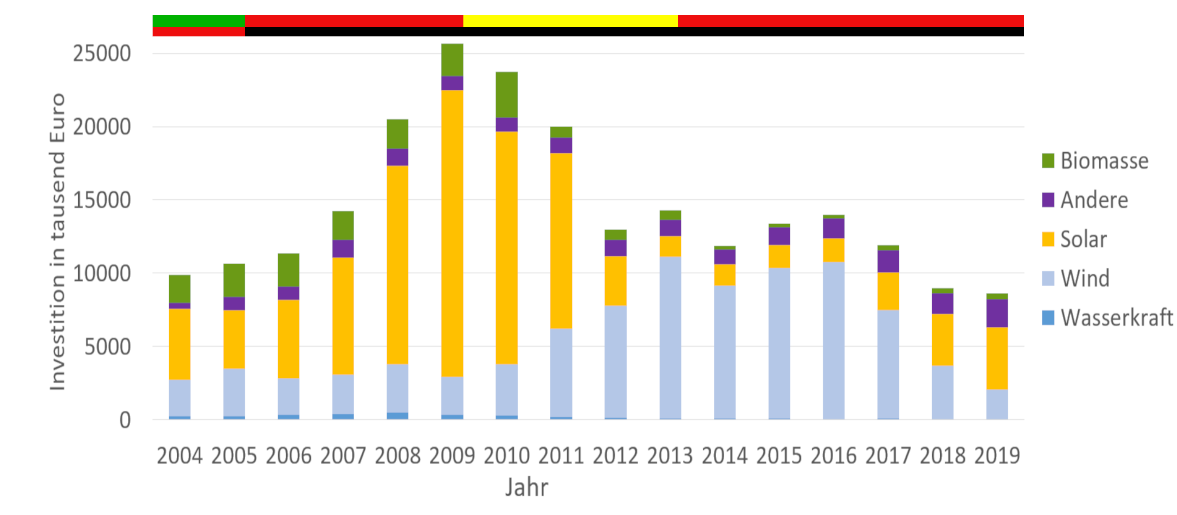
\includegraphics[width=1.2\textwidth]{images/dia_2.png}
    \label{fig:dia-invest}
\end{figure}

Das letzte Diagramm von Abbilding \ref{fig:dia-erz} zeigt die Verteilung der Stromerzeugung  in Deutschland im Zeitraum von 2004 bis 2020. Es ist zu erkennen, dass die Stein- und Braunkohle sowie Kernenergie über die Jahre hinweg sinken und dafür die Windenergie gestiegen ist. Solarenergie, Wasserkraft und Biomasse sind über den Zeitraum leicht gestiegen. 

\begin{figure}[!ht]
    \caption{Erzeugungsverteilung}
    \centering
    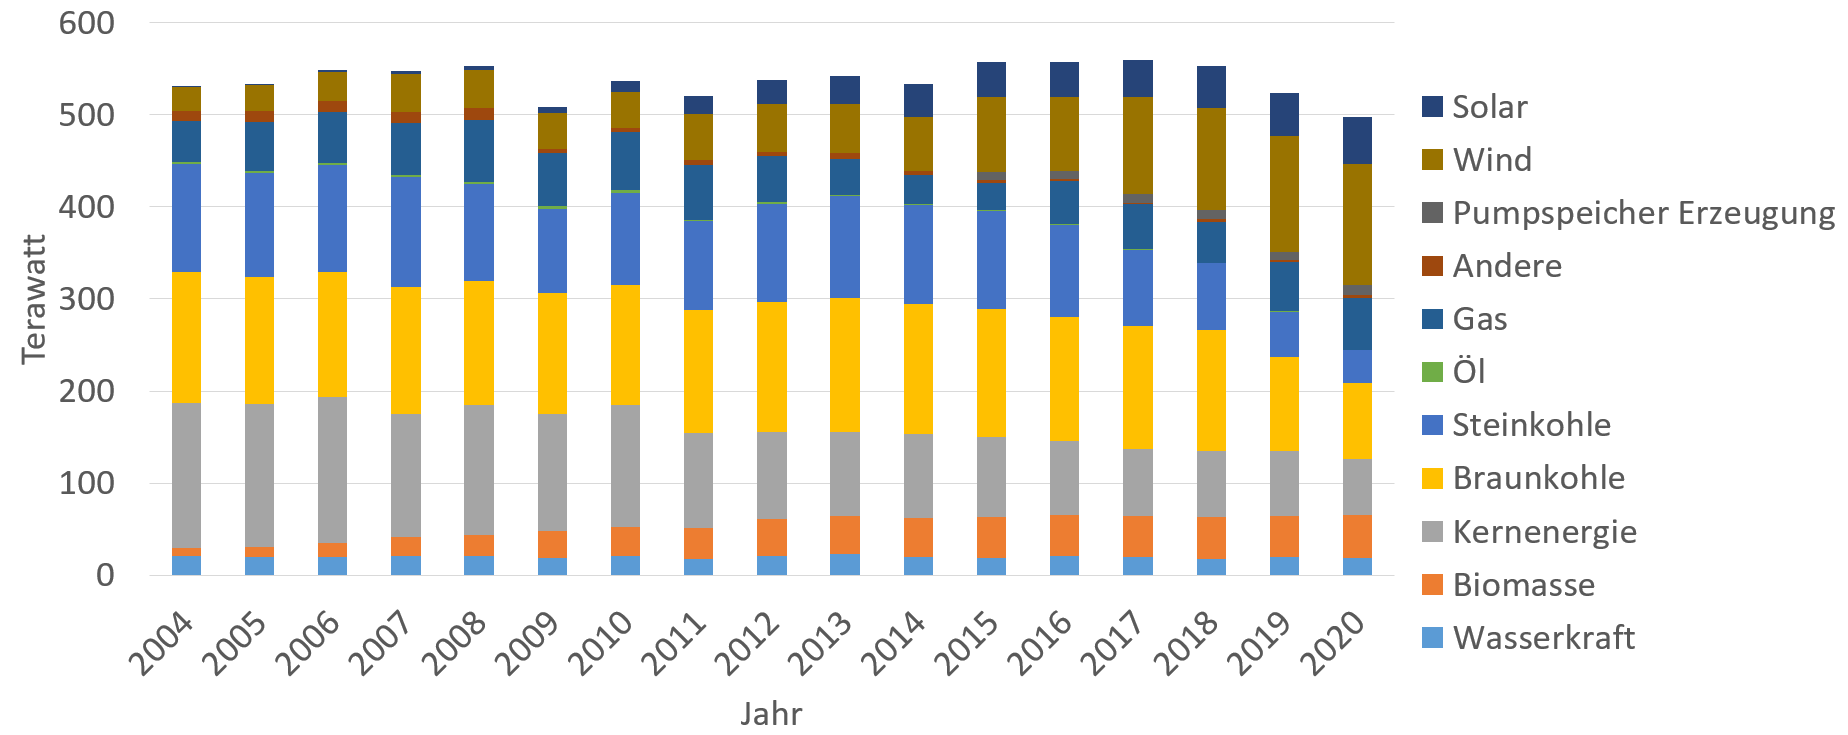
\includegraphics[width=1.2\textwidth]{images/dia_3.png}
    \label{fig:dia-erz}
\end{figure}

\newpage

    \section{Poster}
    
Ein Poster sollte zur Vorstellung der Forschungsfrage und des Zwischenstandes erstellt werden. Diese sollte den Titel, die Forschungsfrage, die Orthologie sowie (falls gegeben) die SPARQL-Anfragen. Zusätzlich sollten das Design der HTWK übernommen werden sowie Daten zum Kurs und einen Link für ein mögliches GIT-Repository mit auf das Posten platziert werden. Um die zusammengesammelten Daten bereits vorzustellen wurden die Daten in eine Exceltabelle gespeichert und als Diagramm ausgegeben. Dabei wurden die Wahlergebnisse und die Gesamt-Investitionshöhe in erneuerbare Energien im Zeitlichen verlauf wurden als X-Y Diagramm dargestellt. Zusätzlich wurde über diesen Diagrammen die gewählte Bundesregierung als Farben dargestellt, welche zu der Zeit (Jahr), die Mehrheit hatten. 

Es ist schon zu erkennen, dass ab 2009 die Bundesregierung (CDU-SPD) wesentlich weniger Geld in erneuerbare Energien investiert hatte als noch zuvor. In diesem Zeitraum hatten die GRÜNEN auch einen wesentlich höheren Anteil in den Wahlergebnissen. 

Somit hat die Bundesregierung es immer mehr der Privatwirtschaft zur Aufgabe gemacht, in erneuerbare Energien zu investieren, da der Anteil der Produktionsmenge zwar stetig steigt, aber die Investitionen stetig sanken. Auch sanken die Investition in Solarkraft und Wasserkraft ab 2009 stark ab. Das Posten kann in Abbildung \ref{fig:poster} betrachtet werden.

\begin{figure}[!ht]
    \caption{Fertiges Poster}
    \centering
    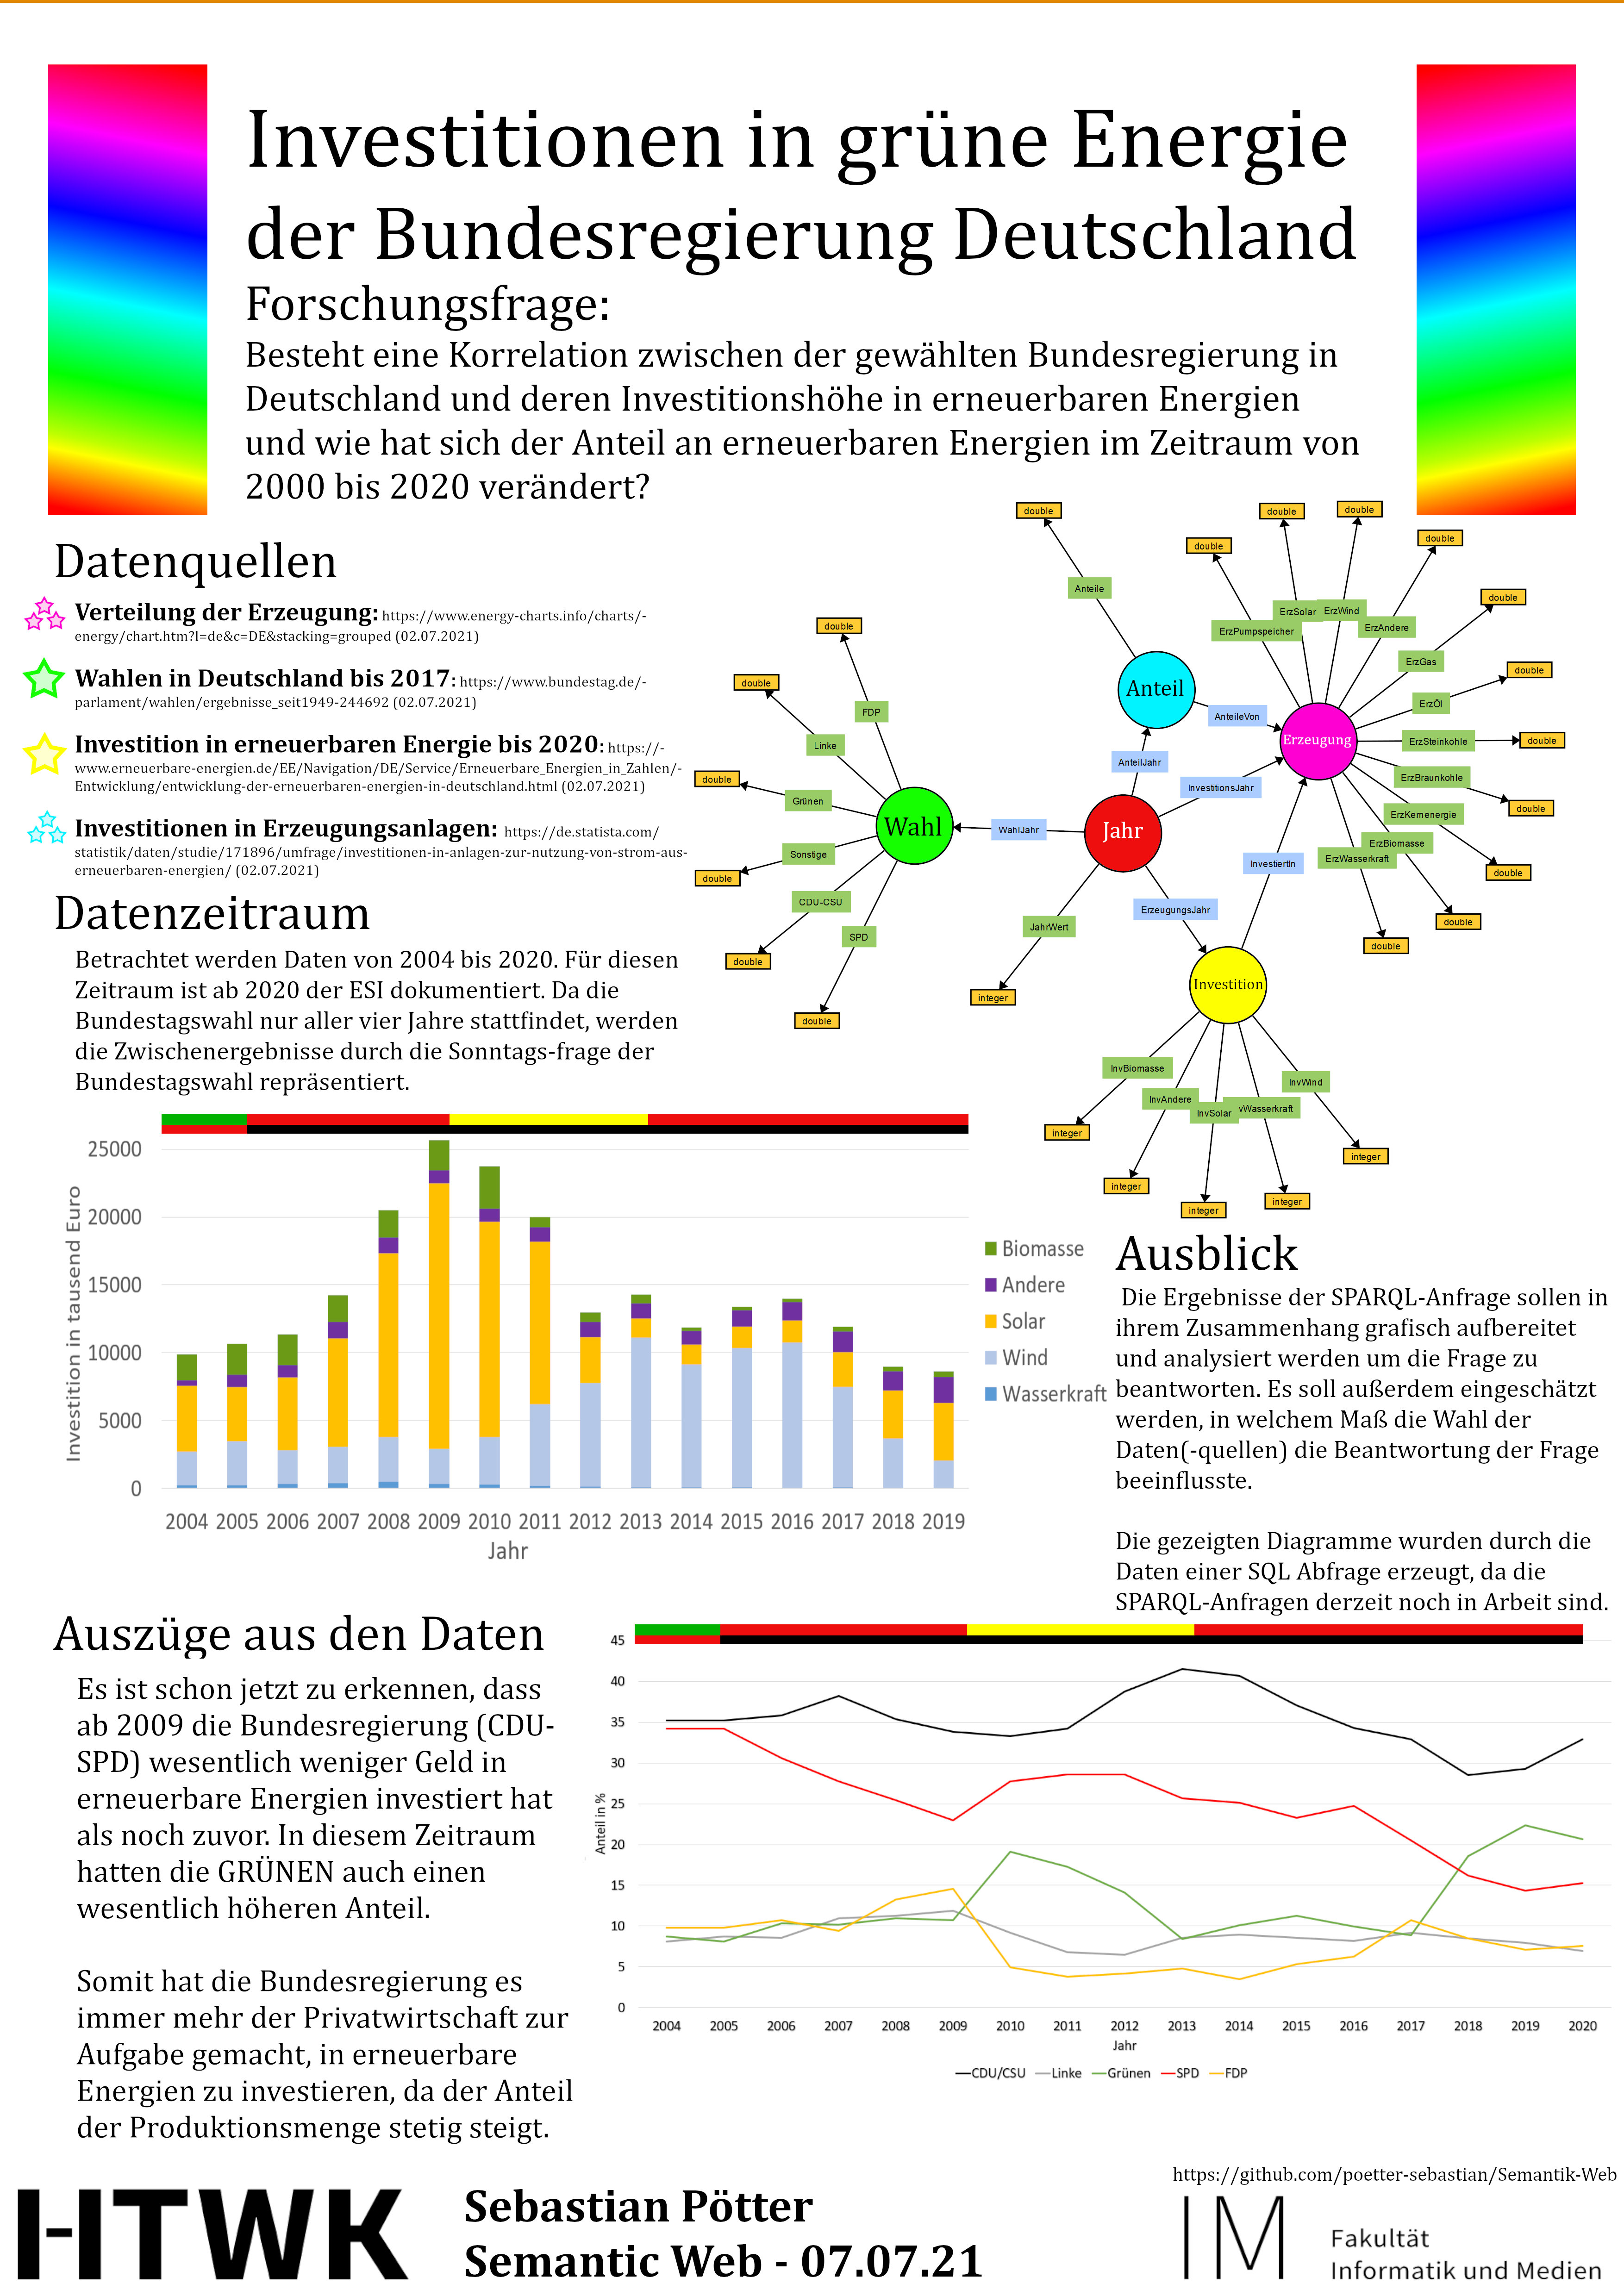
\includegraphics[width=1\textwidth]{images/poster.jpg}
    \label{fig:poster}
\end{figure}

    \section{Lernerfahrungen und Auswertung}

Bis zu diesem Modul wusste ich gar nicht, dass es RDF bzw. SPARQL Abfragen überhaupt gibt. Da ich viel mit Datenbanken mache und mich gut mit SQL-Abfragen auskenne. Den Vorgang von den Rohdaten zu der SPAQL-Abfrage zu kommen ist leider etwas kompliziert gewesen, da wir in der Vorlesung, dieses Thema erst sehr spät behandelt haben. Trotzdem konnte ich viele neue Dinge in Erfahrung bringen und ich sehe jetzt auch Vorteile gegenüber von SQL-Abfragen, welche immer genaue Tabellenquelle benötigen, nicht wie bei SPAQL-Abfragen, wo dies mit der Orthologie bewerkstelligt wird. Durch dieses Fach konnte ich mir ein grobes Verständnis darüber verschaffen, wie eine RDF-Umwandlung funktioniert und wie man diese Daten dann abfragen kann. Zusätzlich war es nochmals eine gute Übung ein Poster zur Darstellung der Forschungsfrage und der momentanen Werte anzufertigen. Genauso ist die Vorstellung von 'Semantik Web' als Teilgebiet der Informatik, welche sich mit der Verknüpfung von Information beschäftigt, wie auch der Möglichkeit der Lesbarkeit von Informationen durch Software. Auch konnte meine Forschungsfrage gut beantworten und habe bemerkt, dass die Bundesregierung viel zu wenig zum Klimaschutz beträgt, als sie eigentlich könnte. Dies kann man auch anhand der Investitionshöhe betrachten, welche seit 2009 sinkt. Es besteht scheinbar ein Zusammenhang von der gewählten Bundesregierung und der Investitionshöhe in erneuerbare Energien. Es sollten dennoch noch weitere Daten in Betracht gezogen werden um diese Annahme zu bestärken. 

    \section{Zusammenfassung}

Die Forschungsfrage konnte mit Daten, welche selbständig aus mindestens drei Quellen gesucht und bereinigt wurden, bearbeitet werden. Dabei wurden Tools benutzt, welche die Daten aus den Bild-Daten beziehungsweise CSV-Format in ein RDF-Format konvertierte, womit dann SPAQL-Anfragen gestellt werden konnten. Diese Anfragen wurden dazu benutzt um Diagramme zu zeichnen und möglichst so zu Gestalten, dass diese die Forschungsfrage beantworten. Dieses Projekt konnte erfolgreich umgesetzt werden und das Teilgebiet, des 'Semantik Web' konnte gut und lehrreich vorgestellt werden.

\end{document}